\documentclass{article}
\usepackage[utf8]{inputenc}
\usepackage{version}
\usepackage{bbold}
\usepackage[tbtags]{amsmath}
\usepackage{amssymb,amsthm}
\usepackage{mathrsfs}
\usepackage{graphicx}
\usepackage{capt-of}
\usepackage{placeins}
\usepackage{caption}
\usepackage{adjustbox}
\usepackage{xcolor}
\usepackage{mathabx}
\usepackage{tkz-tab}
\usepackage{float}
\usepackage{multicol}
\usepackage{enumitem}
\usepackage[many]{tcolorbox}
\newtcolorbox{box_thm}{colback=white!100,colframe=black!100,enhanced}

\newenvironment{Dev}{\begin{box_thm}}{\end{box_thm}}
%\usepackage[all]{xy}

%\usepackage{enumerate}
\usepackage[left=3cm,right=3cm,top=2cm,bottom=2cm]{geometry}
\newtheorem{prop}{Proposition} %[section]
\newtheorem{Cours}[prop]{Cours}
\newtheorem{exo}[subsubsection]{Exercice}
\newtheorem{ques}[prop]{Question}
\newtheorem{cor}[prop]{Corollaire}
\newtheorem{conj}[prop]{Conjecture}
\newtheorem{axi}[prop]{Axiome}
\newtheorem{fait}[prop]{Fait}

\newtheorem*{axi*}{Axiome}

\theoremstyle{definition}
\newtheorem{dfn}[prop]{Définition} %[section]
\newtheorem{exm}[prop]{Exemple}
\newtheorem{contrex}[prop]{Contre-exemple}
\newtheorem{obj}[prop]{Objectif}
\newtheorem{rap}[prop]{Rappel}
\newtheorem{nota}[prop]{Notation}
\newtheorem{app}[prop]{Application}
\theoremstyle{remark}
\newtheorem{rem}[prop]{Remarque}

\renewcommand{\thesection}{\Roman{section}}

\def \N {\mathbb{N}}
\def \R {\mathbb{R}}
\def \U {\mathcal U} % ouverts
\def \V {\mathcal V}
\def \B {\mathcal B} % bases par exemple
\def \L {\mathcal L} % applications linéaires
\def \C {\mathbb{C}}
\def \S {\mathcal{S}}
\def \F {\mathcal{F}}

\renewcommand{\phi}{\varphi}
\newcommand{\derpar}[2]{\frac{\partial #1}{\partial #2}} % der partielles
%\DeclareMathOperator{\dd}{d} % d droit
\newcommand{\dd}[1]{\mathop{\mathrm d #1}}
\DeclareMathOperator{\Jac}{Jac}
\DeclareMathOperator{\Mat}{Mat}
\DeclareMathOperator{\Hess}{Hess}
\DeclareMathOperator{\Tr}{Tr}
\DeclareMathOperator{\Com}{Com}
\def \tp{^t \!}
\newcommand{\fonction}[4]{
    \left. %\{
    \begin{array}{c l l}
       #1 & \to & #2 \\
       #3 & \mapsto  & #4
    \end{array}
    \right.
}
\newcommand{\nfonction}[5]{ % fonction nommée
    \left. %\{
    \begin{array}{c c l l}
       #5 : & #1 & \to & #2 \\
       & #3 & \mapsto  & #4
    \end{array}
    \right.
}
\newcommand{\ps}[2]{\langle #1 \mid #2 \rangle}

\begin{document}
\title{\vspace{-2cm}\LARGE Modélisation de la consommation électrique et de la température à Tetouan (Maroc)}
\author{Ravier Lancelot - Combelles Martin}
\maketitle
\section{Introduction}
La consommation énergétique et les variations de température sont deux phénomènes supposés interdépendants qui jouent un rôle crucial dans la gestion des ressources et la planification des infrastructures. La température influencerait directement la demande énergétique, notamment à travers des besoins en climatisation lors des épisodes de chaleur. Comprendre cette relation et modéliser ces dynamiques est essentiel pour anticiper les pics de consommation, optimiser la production d'énergie et réduire les coûts associés.\newline 

L'objectif de cette étude est d'analyser la consommation énergétique en fonction des variations de température durant la période estivale (Juillet-Aout) et d'explorer notamment comment les modèles de lissage exponentiel (comme Holt-Winters) et les modèles SARIMA peuvent être utilisés pour prédire la demande énergétique et les fluctuations climatiques. Enfin, cette dernière sera l'occasion de s'intéresser à plusieurs moyens de calcul de corrélation entre la demande en énergie et les variations de température.
\section{Données}
Les données analysées dans le cadre de ce projet ont été relevées en 2017 dans la ville de Tetouan, au nord du Maroc (10375 km², estimation à 583374 habitants en 2017). Localisée le long de la mer mediterranée, la température est élevée et l'atmosphère est sèche  durant la période d'été.\newline

Ces données contiennent $n = 52416$ relevés qui, toutes les 10 minutes, fournissent les informations (variables) suivantes : 
\begin{itemize}
    \item $Datetime$ : la date et l'heure ;
    \item $Temperature$ : la température (°C) ;
    \item $conso$ : la consommation électrique (en kWh).
\end{itemize}
Afin de faciliter l'analyse, les données de consommation d'énergie provenant des trois fournisseurs existants (Zone1, Zone2, Zone3) ont été rassemblées en une seule mesure ($conso$) décrivant la consommation totale, en KWh, pour la ville de Tetouan. Aussi, nous allons rassembler les données par heures, afin d'avoir $24$ mesures pour une journée, puis trier les données pour ne garder que la période estivale (Debut : 01/07, fin : 31/08) donnant $T = 63$ $[1:63]$ jours et $t=1488$ mesures au total.
\FloatBarrier
\begin{figure}[!h]
    \centering
    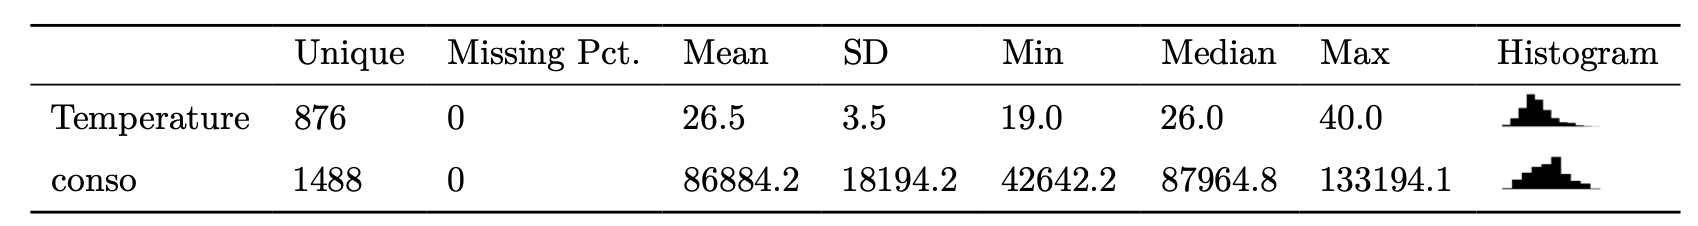
\includegraphics[width=1\linewidth]{fig1.png}
    \caption{Description des variables $Temperature$ et $conso$}
    \label{fig:enter-label}
\end{figure}
L'analyse sera séparée en trois temps : 
\begin{enumerate}
    \item l'analyse de la variable $Temperature$ ;
    \item  l'analyse de la variable $conso$ ;
    \item l'analyse de la corrélation entre les deux mesures.
\end{enumerate}
\newpage
\section{Analyse des séries temporelles}
\subsection{Temperature}
Commençons par décomposer la série temporelle (fig.2) associée à la température que nous noterons $st\_temperature$ :
\FloatBarrier
\begin{minipage}{.5\textwidth}
\hspace{-1cm}
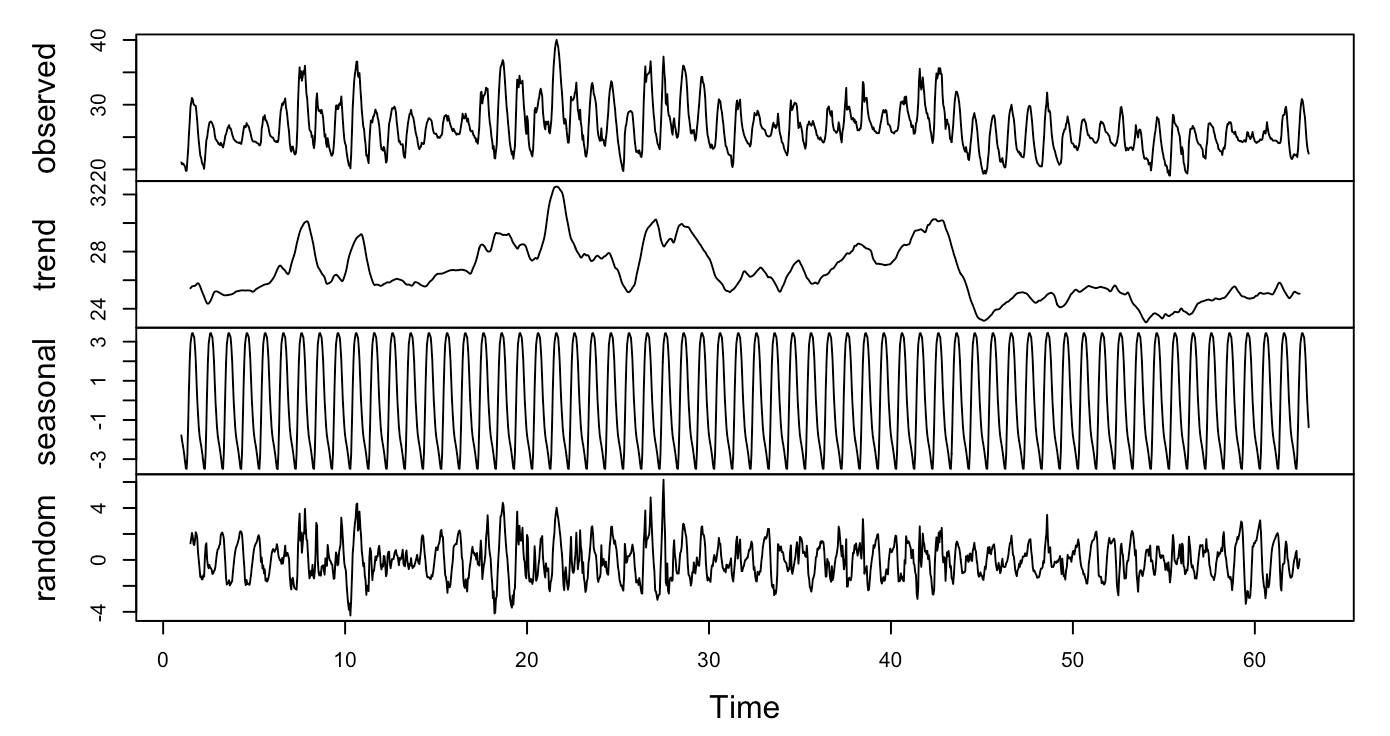
\includegraphics[width=0.95\linewidth]{fig2.png}
    \captionof{figure}{Décomposition de $st\_temperature$}
    \label{fig:enter-label}
\end{minipage}
\begin{minipage}{.5\textwidth}
    \begin{itemize}
    \item La tendance semble linéaire : malgré les fluctuations visibles, la période estivale analysée donne l'intuition de températures relativement constantes durant les deux mois sélectionnés.  
    \item Une saisonnalité journalière semble se dessiner : l'intuition derrière cette analyse est que malgré une tendance constante, les températures baissent la nuit avant de remonter en journée (pic haut vers 15, pic bas vers 7h).
    \end{itemize}
\end{minipage}
\newline
\\
Comme la tendance a une amplitude de moins de 10°C sur une période de plus de 60 jours, il ne semble pas nécessaire de modéliser la tendance autrement que par la température moyenne de cette dernière sous peine de complexifier le modèle. De plus, les moyennes hebdomadaires ne varient que très peu ( elles sont comprises entre 24.95 et 28.46 °C). Néanmoins, on peut essayer d'ajuster un modèle linéaire. Sans grande surprise, le coefficient directeur de la droite de régression est de l'ordre de $-10^{-3}$. Nous ferons le choix de ne pas modéliser la tendance pour le moment : lorsque nous effectuerons le test de kpss de stationnarité, celui-ci montrera s'il est nécessaire de différencier ou non la série temporelle afin de garantir la stationnarité des résidus.
Maintenant, analysons l'ACF de la série temporelle afin de pouvoir sélectionner et paramétrer au mieux le modèle final :\newline \\
\begin{minipage}{.5\textwidth}
\hspace{-1cm}
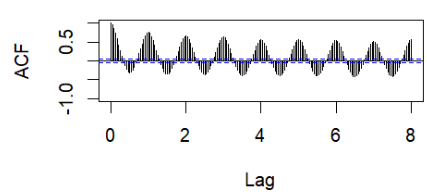
\includegraphics[width=0.95\linewidth]{fig3.png}
    \captionof{figure}{ACF de $st\_temperature$}
    \label{fig:enter-label}
\end{minipage}
\begin{minipage}{.5\textwidth}
    La forme de sinusoïde de l'ACF montre une saisonnalité claire à chaque lag (toutes les 24h) (ce qui vient confirmer l'intuition de départ). Ainsi, nous allons commencer par modéliser notre série avec un modèle SARIMA en ajoutant une différenciation saisonnière (D=1). Le test kpss, qui teste l'hypothèse $\mathcal{H}_0$ : \textit{"les résidus sont stationnaires"} donnera ensuite une indication sur la stationnarité ou non des résidus du modèle, avec la particularité de détécter ausis la présence de saissonalité/tendance résiduelle.
\end{minipage}
\newline
\\
Représentons l'ACF et le partial ACF de la série brute une fois avoir appliqué une différenciation saisonnière :
\FloatBarrier
\begin{minipage}{.5\textwidth}
\hspace{-1cm}
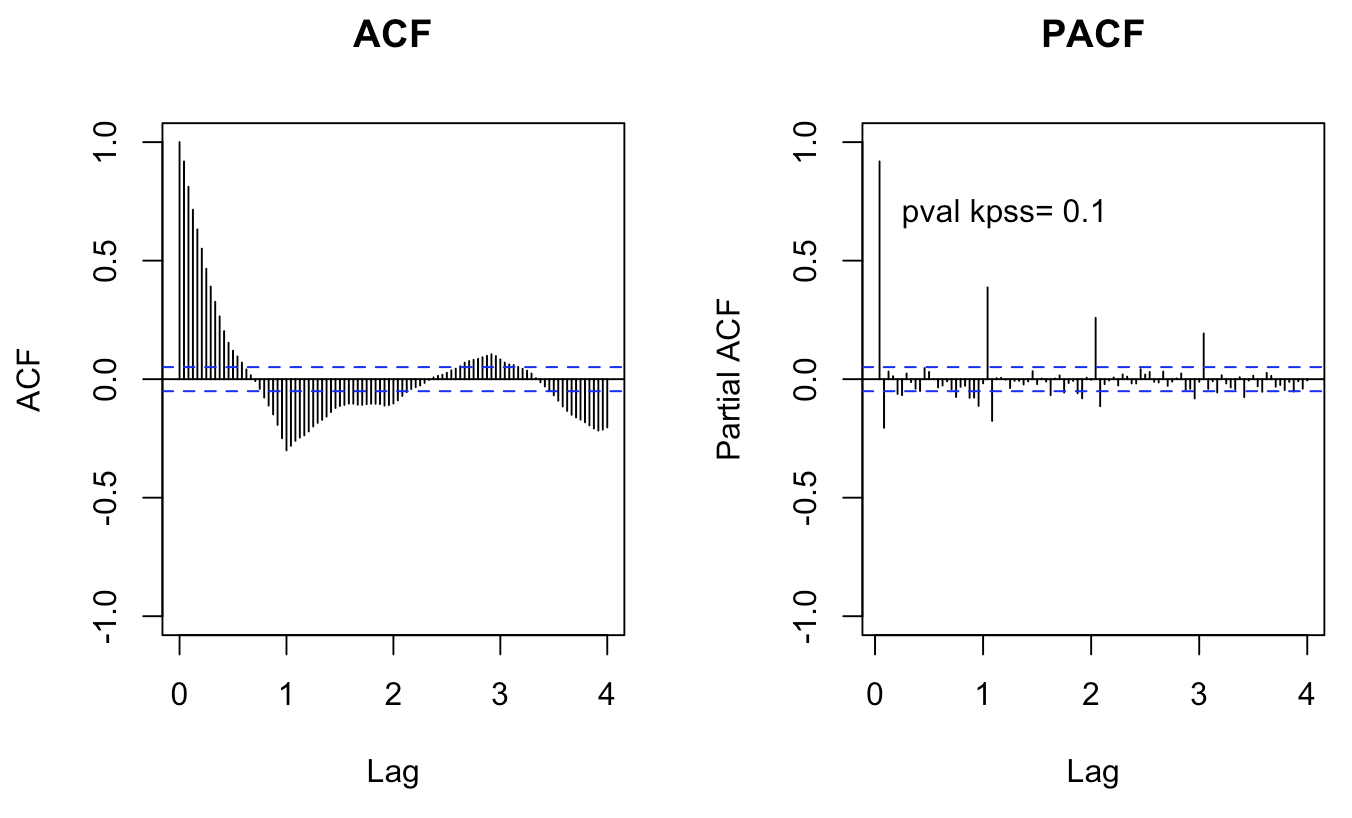
\includegraphics[width=0.95\linewidth]{fig4.png}
    \captionof{figure}{ACF et PACF - ARIMA(0,0,0)(0,1,0)[24]}
    \label{fig:enter-label}
\end{minipage}
\begin{minipage}{.5\textwidth}
    \begin{itemize}
        \item L'ACF montre que la différenciation saisonnière appliquée à la série a bien permis d'affaiblir l'effet de la saisonnalité (le pattern sinusoïdal a disparu)
        \item le test kpss (non-significatif) indique que les résidus du modèle sont stationnaires : en plus de la suppression effective de la saisonnalité par différenciation, le test montre aussi qu'il n'est pas nécessaire de modéliser la tendance par différenciation car celle-ci n'est pas présente dans les résidus (elle n'influence pas la stationnarité dans ce cas)
        \item le fait que l'ACF et le PACF sont significatifs à chaque lag pousse à appliquer un terme auto-régressif (PACF) et de moyenne mobile (ACF) tout deux saisonniers (P = 1, Q = 1)
        \item sur le PACF, les deux premiers pics sont significatifs, ce qui pousse à prendre un terme auto-régressif d'ordre 2 (p = 2).
    \end{itemize}
\end{minipage}
\newline
\\
Le modèle retenu est donc un SARIMA(2,0,0)(1,1,1)[24].\newline
Vérifions alors l'ACF, le partial ACF, la blancheur (test de Box-Ljung) ainsi que la normalité des résidus (QQ-plot).
\FloatBarrier
\begin{figure}[!h]
    \centering
    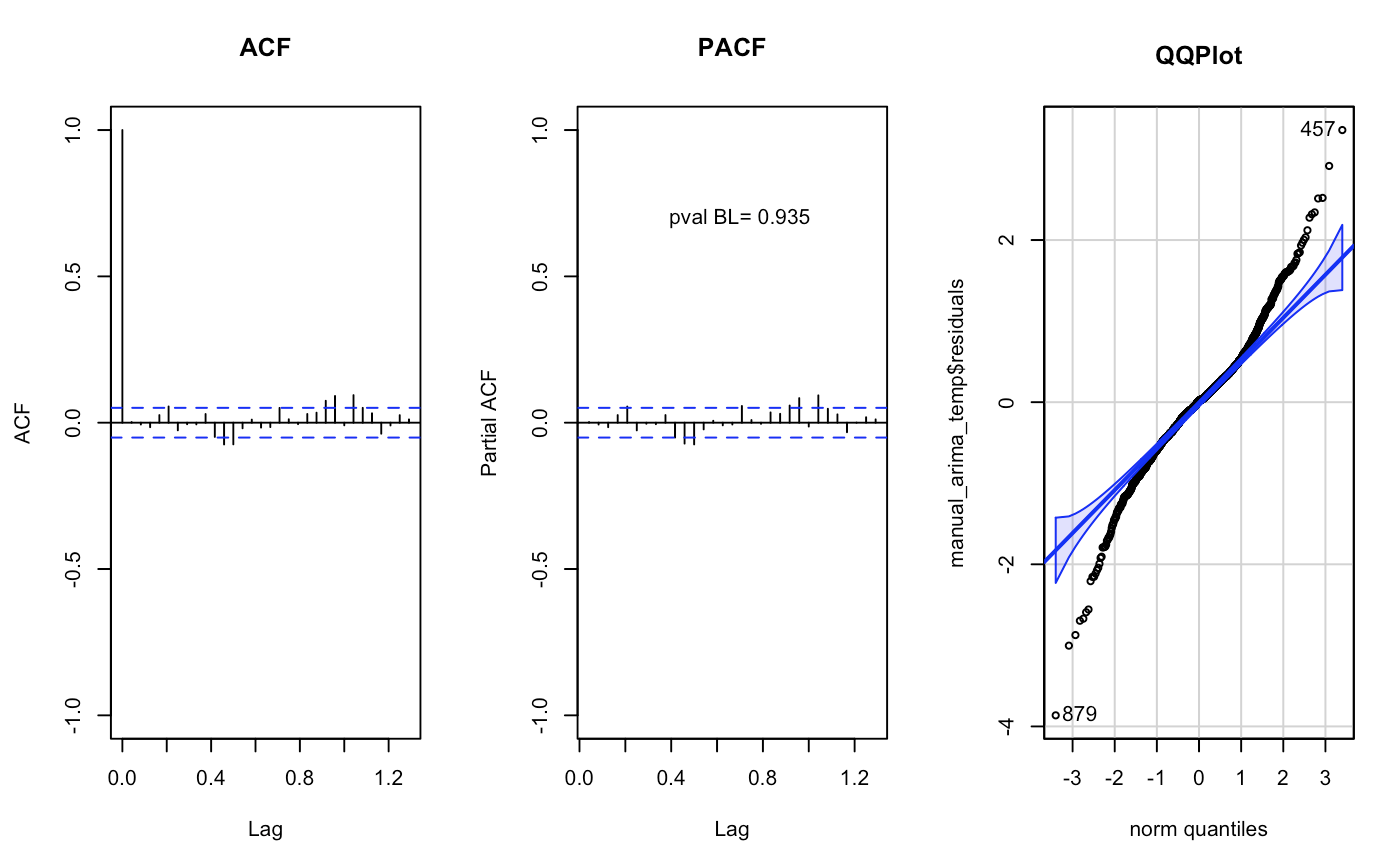
\includegraphics[width=0.6\linewidth]{fig5.png}
    \caption{ACF, PACF et QQ-plot associés aux résidus du modèle SARIMA(2,0,0)(1,1,1)[24]}
    \label{fig:enter-label}
\end{figure}
Selon les deux premiers graphiques, la quasi-totalité des variations significatives ont été captées par le modèle. Le test de Box, qui teste l'hypothèse $\mathcal{H}_0$ \textit{"la série est un bruit blanc"}, est significatif et donc vient confirmer cette intuition en montrant que les résidus du modèle sont bien un bruit blanc.\newline
Après analyse, les perturbations du modèle semblent homoscédastiques : l'intuition sur la non-variabilité des température moyennes durant ces deux mois viennent confirmer l'analyse, même si les résidus ne sont pas parfaitement homoscédastiques (test de Breuch-Pagan d'heteroscédasticité significatif qui teste l'hypothèse $\mathcal{H}_0$ : \textit{"les résidus sont homoscédastiques"}). De plus, les résidus du modèle ne suivent pas une loi normale : la distribution des résidus reste fortement leptokurtique et asymétrique à droite. 

En réalité, ces deux hypothèses ne seraient nécessaire que pour construire des intervalles de confiance sur les prédictions. Le fait qu'elles ne soient pas vérifiées ne changent en rien la pertinence du modèle trouvé. Comme nous connaissons les températures durant les mois suivants, ces intervalles ne sont pas utiles. A la place, nous avons choisi de tracer la courbe de température les trois premiers jours de septembre et la prédictions sur le même graphe. Ensuite, on calculera le RMSE pour évaluer l'erreur.\newline
\newline
\\
Afin de s'assurer de la pertinence du modèle, nous allons le comparer aux modèles conçus par les algorithmes *auto.arima*, configurés en fonction de l'AIC (critère choisi pour sélectionner le modèle optimal en équilibrant l'ajustement aux données et la complexité du modèle, en privilégiant celui avec l'AIC le plus bas.), et au modèle de lissage exponentiel automatique de Holt-Winters car ce dernier est particulièrement adapté aux séries temporelles présentant des tendances et des saisons comme celle-ci. Comparer SARIMA à Holt-Winters permet d’évaluer si une approche fondée sur la décomposition explicite des composantes (tendance et saisonnalité) améliore la prévision. En effet, alors que SARIMA capture les dépendances temporelles à travers des termes autorégressifs et des moyennes mobiles, Holt-Winters met davantage l’accent sur l’évolution progressive des tendances et des variations saisonnières.

\begin{figure}[!h]
    \centering
    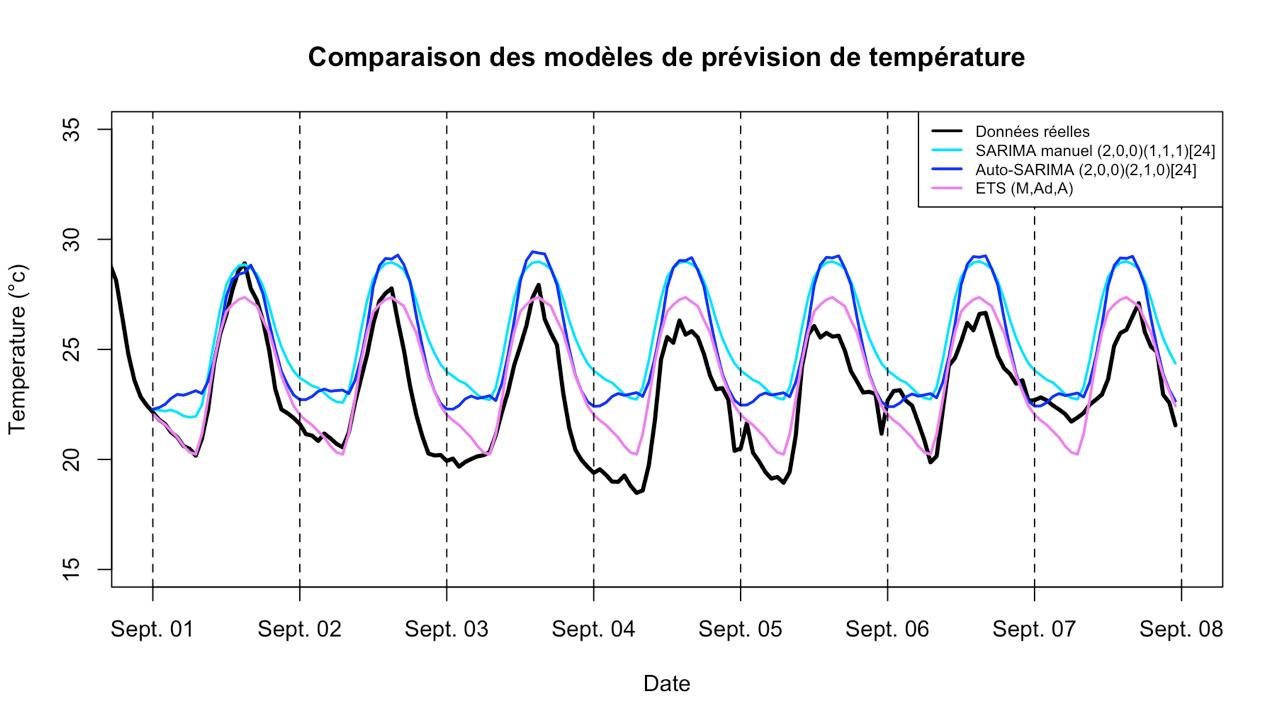
\includegraphics[width=0.75\linewidth]{figtemp.jpg}
    \caption{Comparaison des modèles de prévision de la température}
    \label{fig:enter-label}
\end{figure}
Selon ce graphique, nous pouvons voir que les trois modèles présentent des différences significatives. Ainsi, sur les sept jours
\begin{itemize}
    \item Le modèle manuel ARIMA(2,0,0)(1,1,1)[24] (courbe cyan) capture relativement bien le pic saisonnier du premier jour. Cependant, il surestime
les valeurs dans la période creuse, réagit mal aux chutes abruptes de températures et sa précision lors des pics
hauts décroît fortement lors des jours suivants.
\item Le modèle automatique ARIMA(2,0,0)(2,1,0)[24] (courbe bleu foncé) capture le premier pic de manière similaire au modèle manuel et possède une meilleure adéquation que le modèle manuel lors des chutes abruptes de température. De plus, il est plus précis lors des creux de température. Cependant, il prédit moins bien le premier creux de température et, comme le premier modèle, sa capacité à prédire
des pics et des variation abruptes de température décroît avec le temps.
\item Le modèle ETS (M,Ad,A) (courbe pourpe) considère l'erreur multiplicative, la tendance additive et amortie et la saissonalité additive. Il possède une meilleure précision
dans les creux : il lisse efficacement les variations brutales et ne les surestime pas. Cependant, il sous-estime les trois premiers pics de température (probablement à cause d’une composante saisonnière trop lissée) et sur-estime les quatre derniers pics.
\end{itemize} 
Ainsi, le modèle SARIMA manuel serait plus adapté pour les saisonnalités marquées au détriment des changement brusques. Le modèle SARIMA automatique est plus flexible pour les fluctuations rapides mais toujours sujet au sur-ajustement. ETS excelle pour les tendances lissées et les creux, cependant au détriment des pics de température. Pour finir, aucun de nos modèles n’est performant lorsque l’on dépasse le deuxième jour.
\newpage
Comparons les RMSE pour pouvoir comparer les prédictions des modèles chaque jour.
\FloatBarrier
\begin{figure}[!h]
    \centering
    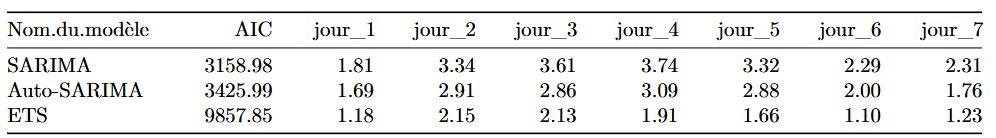
\includegraphics[width=1\linewidth]{fig20.png}
    \caption{RMSE des modèles pour la semaine du 01/09 au 07/09}
    \label{fig:enter-label}
\end{figure}
Le mod\`ele SARIMA manuel (2,0,0)(1,1,1)[24] pr\'esente les valeurs d'AIC (3158.98) et de BIC (3185.42) les plus faibles, indiquant qu'il est le plus parcimonieux parmi les trois. L'Auto-SARIMA (2,0,0)(2,1,0)[24] a des valeurs plus \'elev\'ees (AIC = 3421.59, BIC = 3448.04), sugg\'erant qu'il est moins performant en termes d'ajustement. Enfin, le mod\`ele ETS (M,Ad,A) est le moins satisfaisant avec un AIC de 9857.85 et un BIC de 10017.00, ce qui indique un ajustement sous-optimal aux donn\'ees d’entra\^inement.

\begin{itemize}
    \item Jour 1 : Le mod\`ele ETS (M,Ad,A) offre la pr\'evision la plus pr\'ecise avec un RMSE de 1.18, contre 1.73 pour l'Auto-SARIMA et 1.81 pour le SARIMA manuel. \`A tr\`es court terme, l'ETS semble donc le plus efficace ;
    \item Jours 2 \`a 4 : Le SARIMA manuel affiche des erreurs l\'eg\`erement plus \'elev\'ees (entre 3.34 et 3.74), tandis que l'Auto-SARIMA pr\'esente des erreurs un peu plus faibles (entre 2.94 et 3.13). L'ETS conserve un avantage avec des erreurs plus faibles (entre 2.15 et 1.91), indiquant une meilleure stabilit\'e sur cette p\'eriode ;
    \item Jours 5 \`a 7 : L'ETS maintient de bonnes performances avec des erreurs comprises entre 1.66 et 1.23. L'Auto-SARIMA montre une diminution de l'erreur, ce qui indique une meilleure pr\'ecision \`a plus long terme par rapport au SARIMA manuel, qui conserve des erreurs l\'eg\`erement plus \'elev\'ees.
\end{itemize}

En conclusion, le SARIMA manuel est le mod\`ele le plus \'equilibr\'e : il offre un bon compromis entre performance et complexit\'e gr\^ace \`a ses faibles valeurs de BIC et AIC. Le mod\`ele ETS (M,Ad,A) est le plus pr\'ecis \`a court et moyen terme, mais ses crit\`eres AIC et BIC \'elev\'es indiquent qu'il n'est pas optimal en termes de mod\'elisation. Pour finir, l'Auto-SARIMA est globalement moins performant que le SARIMA manuel, avec des erreurs plus faibles \`a certains moments mais un BIC plus \'elev\'e.


\subsection{Consommation électrique}
Commençons par décomposer la série temporelle $st\_conso$ en tendance, partie saisonnière et partie résiduelle.
\FloatBarrier
\begin{minipage}{.5\textwidth}
\hspace{-1cm}
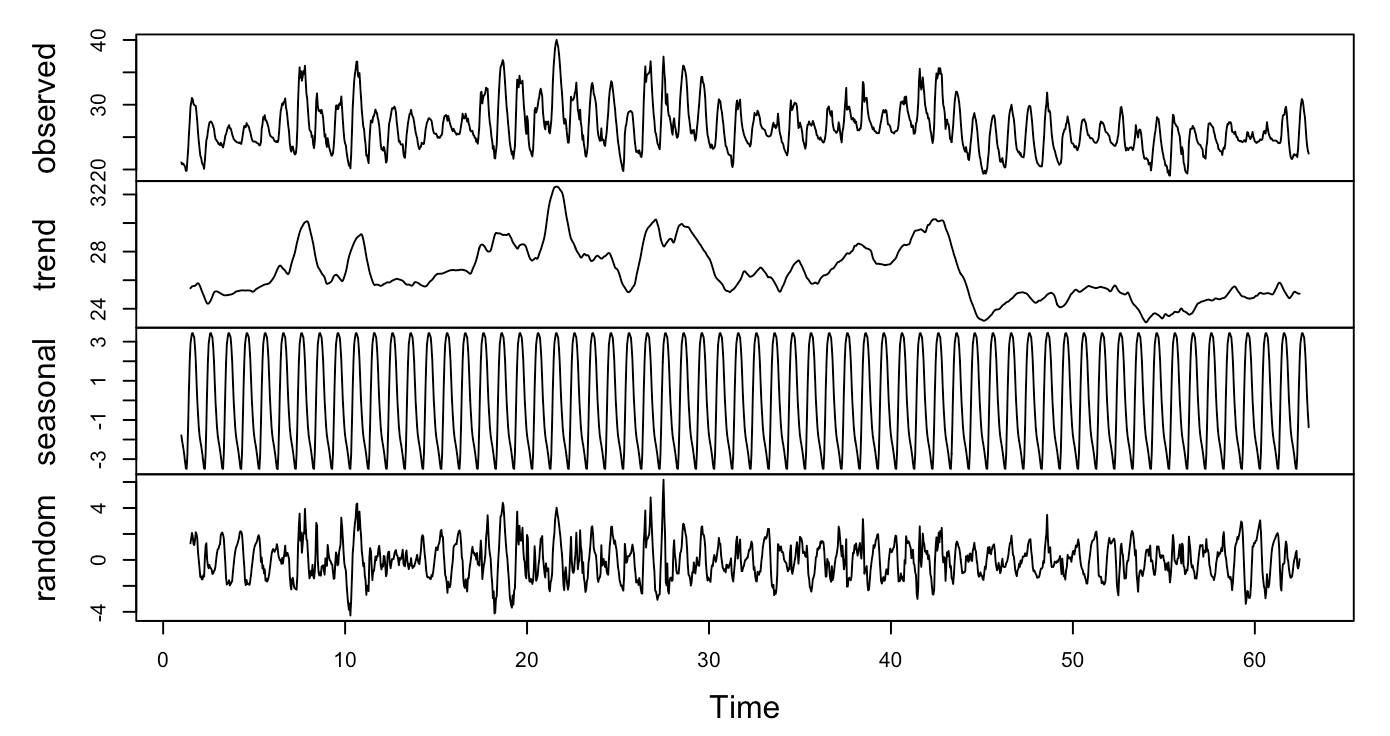
\includegraphics[width=0.95\linewidth]{fig2.png}
    \captionof{figure}{Décomposition de $st\_conso$}
    \label{fig:enter-label}
\end{minipage}
\begin{minipage}{.5\textwidth}
    A partir de la décomposition de $st\_conso$, on observe :
    \begin{itemize}
    \item une tendance comprise entre 70000 kWh et 100000 kWh (étendue de 30000 kWh). Cette dernière est globalement croissante sur le mois de juillet puis décroissante sur le mois d’août
    \item une saisonnalité journalière avec une amplitude de 60000 kWh  (consommation minimale à 6h et maximale à 20h)
    \item une partie résiduelle comprise entre -5000 et 5000 kWh les cinquante premiers jours avec une variance plutôt constante et entre -10000 et 15000 kWh les dix derniers jours (avec une variance qui augmente de jours en jours).
    \end{itemize}
\end{minipage}
\newpage
Le test kpss pour la série non-désaisonnalisée et/ou non différenciée est significatif . On va devoir devoir différencier la série et inclure une différenciation saisonnière qui capteront la partie non-stationnaire de la série (d=1, D=1).\newline

Représentons l'ACF et le partial ACF après avoir appliqué une différentiation et une différentiation saisonnière à la série :
\FloatBarrier
\begin{minipage}{.5\textwidth}
\hspace{-1cm}
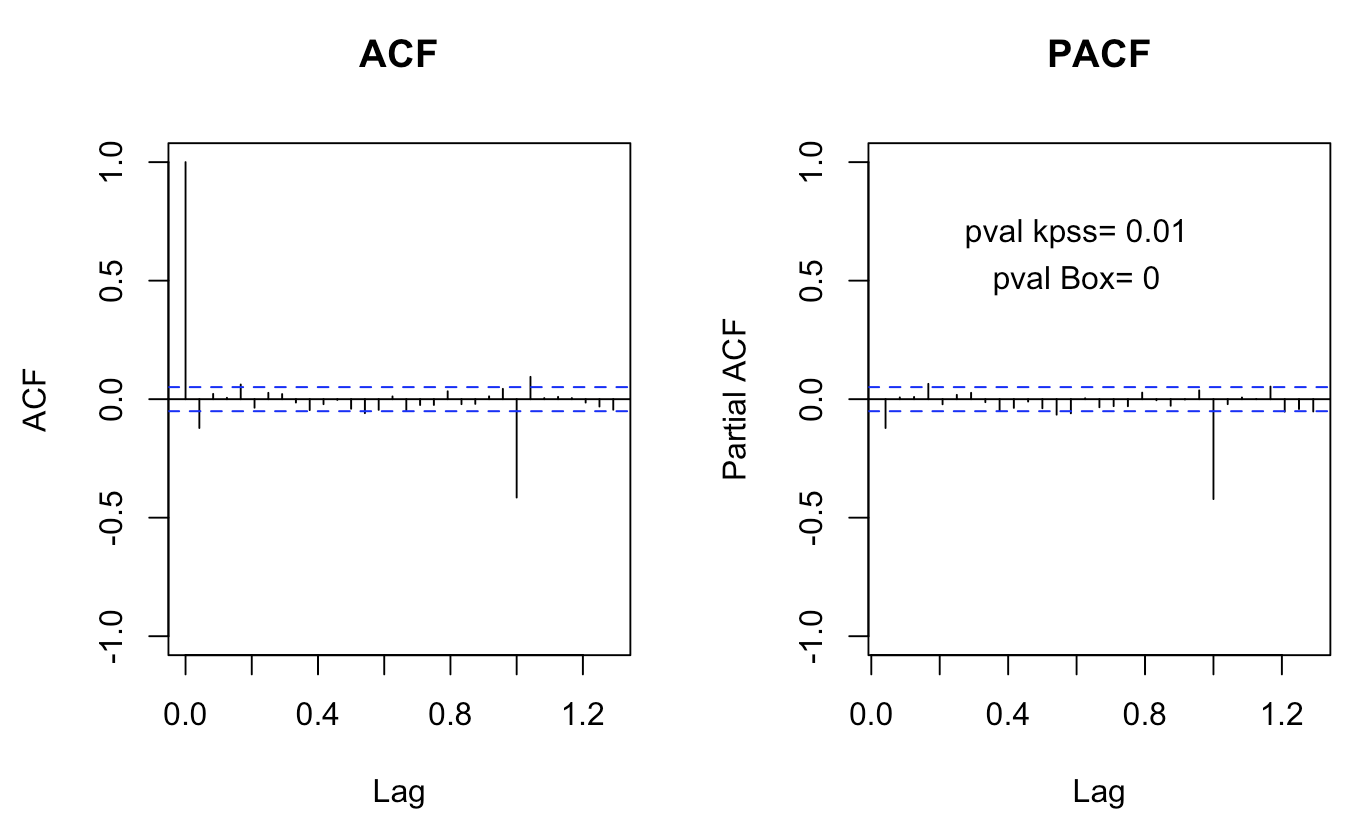
\includegraphics[width=0.95\linewidth]{fig9.png}
    \captionof{figure}{ACF et PACF associés aux résidus ARIMA(0,1,0)(0,1,0)[24]}
    \label{fig:enter-label}
\end{minipage}
\begin{minipage}{.5\textwidth}
    L’ACF et le PACF montrent des pics significatifs à chaque période (tous les 24 pics) montrant ainsi
    une saisonnalité dans les deux graphes. Afin de corriger cela, nous appliquerons un paramètre auto-régressif et de moyenne mobile saisonnier d’ordre 1 (P = 1, Q = 1).\newline
    De plus, on voit que le premier pic du PACF est significatif. Ainsi, nous allons appliquer un terme auto-régressif d’ordre p = 1.\newline\\    
\end{minipage}
\newline
\\
Le modèle retenu est donc un SARIMA(1,1,0)(1,1,1)[24].\newline
Vérifions alors l’ACF, le partial ACF, la blancheur (test de Box-
Ljung) ainsi que la normalité des résidus (QQ-plot).\newline
\FloatBarrier
\begin{minipage}{.5\textwidth}
\hspace{-1cm}
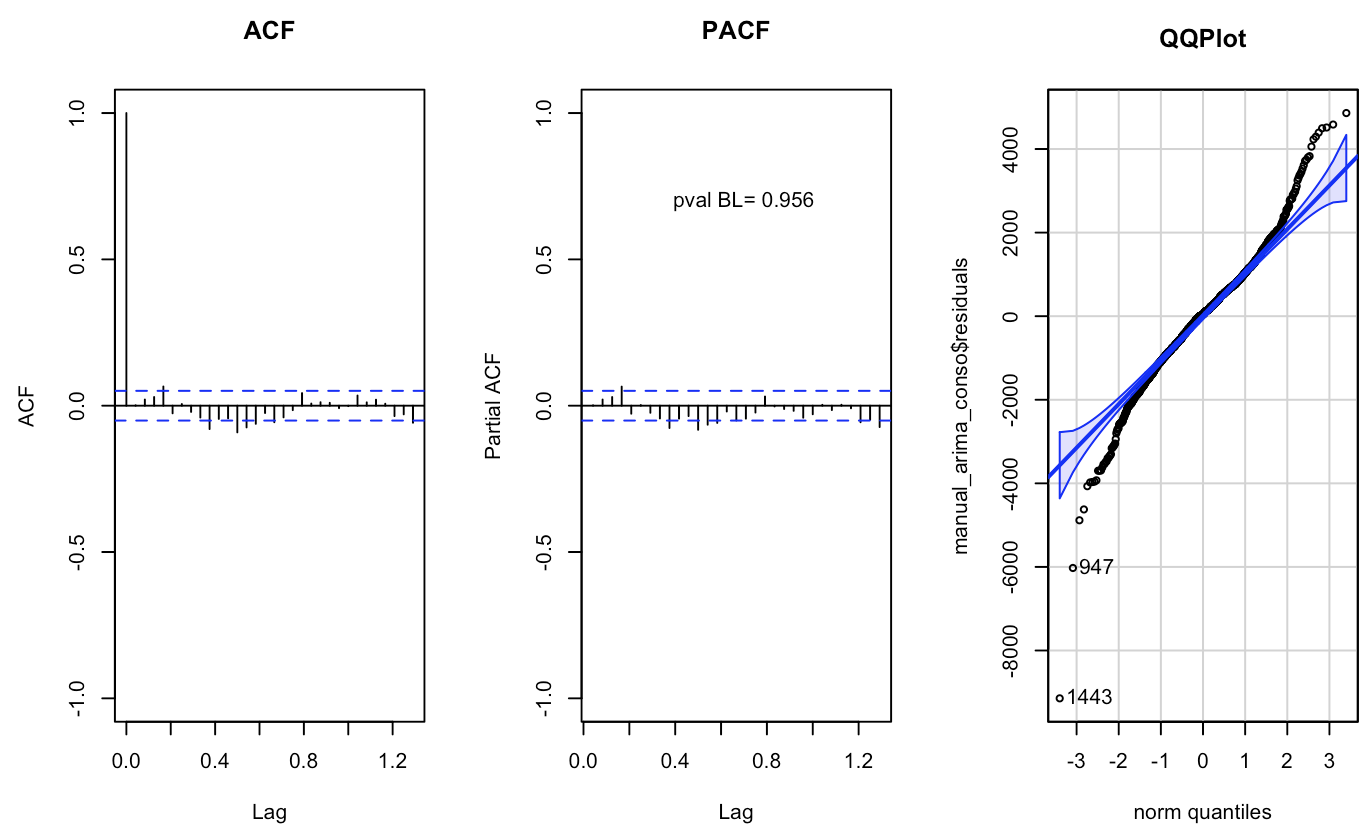
\includegraphics[width=0.95\linewidth]{fig10.png}
    \captionof{figure}{ACF, PACF et QQ-plot associés aux résidus du modèle SARIMA(1,1,0)(1,1,1)[24]}
    \label{fig:enter-label}
\end{minipage}
\begin{minipage}{.5\textwidth}
    Selon les deux graphiques, la quasi-totalité des variation significatives ont été captées par le modèle. Le test de Box vient confirmer cette intuition en montrant que les résidus du modèle sont bien un bruit blanc. Cependant, comme pour $st\_temperature$, les résidus ne suivent pas une loi normale.\newline \\
\end{minipage}
\newline
\\
Comparons le modèle ainsi construit à celui construit automatiquement grâce à la fonction $auto-arima$ et au modèle de lissage exponentiel.
\FloatBarrier
\begin{figure}[!h]
    \centering
    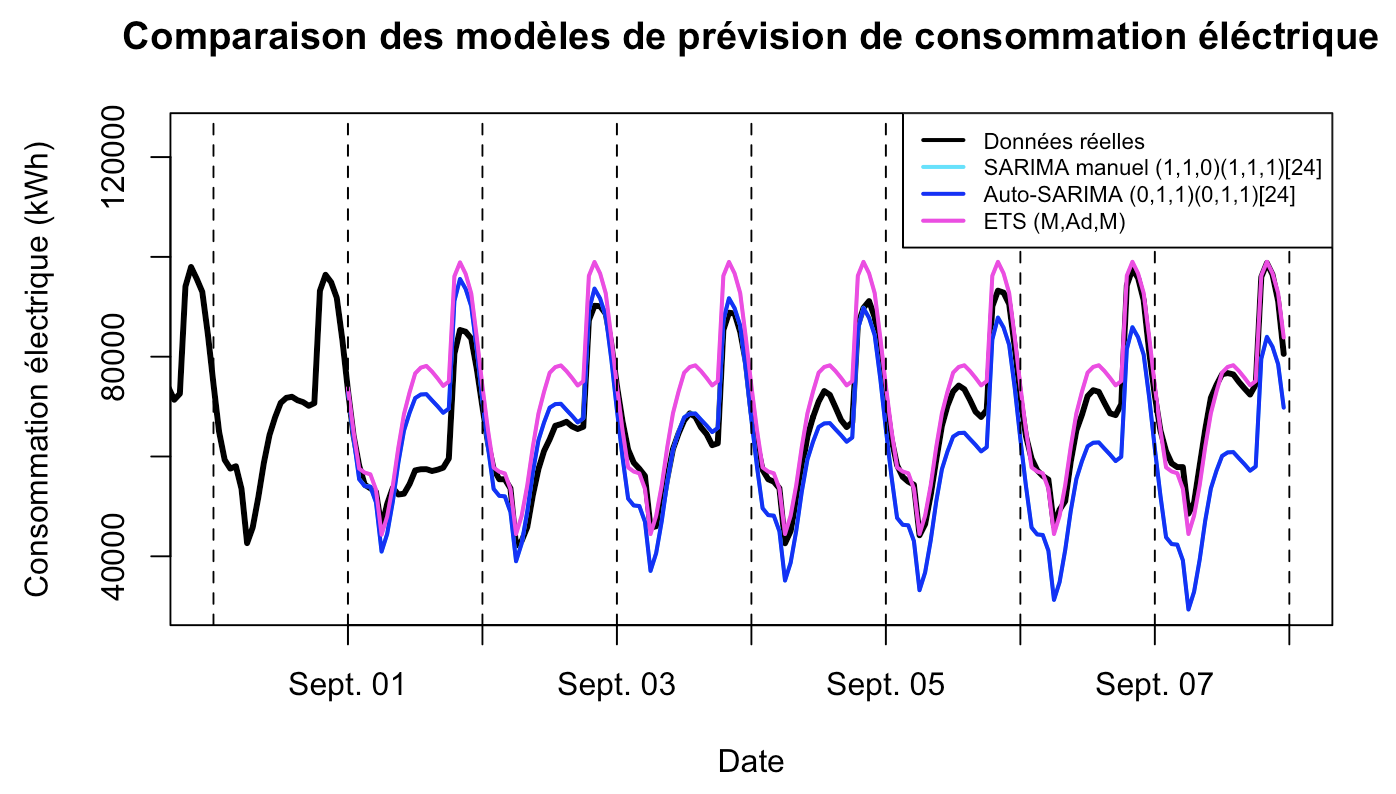
\includegraphics[width=0.65\linewidth]{fig+.png}
    \caption{Comparaison des modèles de prévision de la consommation électrique}
    \label{fig:enter-label}
\end{figure}
Le graphique nous montre un évènement spécial lors du premier jour, évènement absolument pas capté parles modèles de prévisions. Selon ce graphique, on voit que les modèles SARIMA manuel et automatique sont très similaires dans
leurs estimations. 
\begin{itemize}
    \item Modèles SARIMA : Les pics de basses consommations (aux alentours de midi) sont bien estimés lors des deux premiers jours mais de plus plus en plus sous-estimés ensuite. Ils estiment bien les pics hauts (aux alentours de 19h) à partir du jour 2 jusqu'au jour 4 et captent davantage les variations intermédiaires (chute partielle de consommation avant atteinte du pic).\newline
Les variations abruptes sont aussi bien estimées. Cependant, ces deux modèles tendent à sous-estimer les valeurs réelles avec le temps, toute heure confondue.
    \item Modèle ETS (M, Ad, M) : En considérant l'erreur et la saissonalité multiplicative avec la trend additive et amortie, la Le modèle ETS est globalement meilleur que les modèles SARIMA pour estimer les creux de consommation, mais il a tendance à sur-estimer les pics de midi et de 19h, surtout lors des premiers jours. Aussi, malgré une moins bonne estimation des variations intermédiaires et des quatre premiers pics de midi comparé aux deux autres modèles, ETS estime mieux et de manière plus stable la consommation, là où les
modèles SARIMA perdent fortement en précision dans le temps.
\end{itemize}
A court terme, les modèles SARIMA permettent une meilleure estimation des pics de consommation et des periodes creuses, tandis que le modèle ETS a tendance a surestoimer,, sauf lors des pics bas. A moyen et long terme, les pics journaliers montrent qu’ETS surestime moins et suit la tendance globale, tandis que les modèles SARIMA
divergent dans le temps. A partir du jour 6, les modèles SARIMA sous-estiment fortement la consommation en particulier pendant les creux nocturnes et les pics de midi. \newline
Ainsi, le modèle ETS est mieux adapté pour les prévisions nocturnes et au long terme alors que les modèles SARIMA prédit mieux la consommation en journée de J+1 à J+4.\newline \\
On peut comparait les prédictions des différents modèles grâce au RMSE calculé quotidiennement pendant une semaine. 
\FloatBarrier
\begin{figure}[!h]
    \centering
    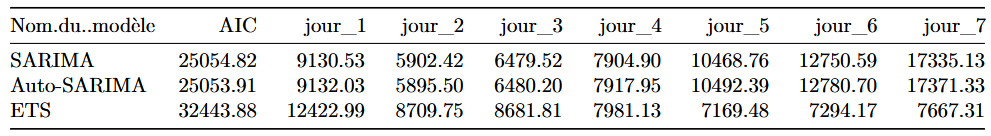
\includegraphics[width=1\linewidth]{fig21.png}
    \caption{RMSE des modèles pour la semaine du 01/09 au 07/09}
    \label{fig:enter-label}
\end{figure}
Comme on le voit sur ce tableau, le modèle ETS est en moyenne moins précis que les modèles SARIMA pour les 4 premiers jours (différence d'erreur de $3000$ KWh), mais cette tendance s'inverse ensuite et ETS devient largement plus précis que les modèles SARIMA (diférence d'erreur moyenne de $10000$ KWh à j+7).
Le SARIMA manuel (1,1,0)(1,1,1)[24] et l'Auto-SARIMA (0,1,1)(0,1,1)[24] affichent des valeurs d'AIC et BIC tres proches (AIC = 25054, BIC = 25070), indiquant des performances similaires en termes de modélisation. En revanche, l'ETS (M,Ad,A) est nettement moins performant avec un AIC de 32443.88 et un BIC de 32603.03, ce qui suggere un moins bon ajustement aux donnees d'entrainement.
\begin{itemize}
    \item Jour 1 : Les deux modèles SARIMA sont très proches, avec une erreur d’environ 9130, tandis que l’ETS affiche une erreur nettement plus élevée (12422.99), ce qui indique une moins bonne précision à court terme.
    \item Jours 2 à 4 : L’Auto-SARIMA et le SARIMA manuel continuent d'afficher des erreurs similaires (autour de 5900-7900), tandis que l’ETS reste en retrait avec des erreurs plus élevées (8709.75 à 7981.13).
    \item Jours 5 à 7 : L’écart entre les modèles SARIMA et l’ETS devient encore plus marqué. L’ETS montre une amélioration progressive avec une erreur de 7667.31 au jour 7, mais reste bien au-dessus des erreurs des modèles SARIMA, qui augmentent significativement pour atteindre environ 17350.
\end{itemize}
En conclusion, le modèle SARIMA manuel et l’Auto-SARIMA offrent des performances équivalentes, avec des critères d’information très proches et des erreurs de prévision similaires. Le modèle ETS est clairement moins performant avec un AIC et un BIC très élevés et une erreur RMSE plus importante sur presque toute la période. pour des prévisions à j+1/2/3/4, les modèles SARIMA sont préférables, mais au long terme, leurs erreurs augmentent fortement. Ainsi, le choix entre le SARIMA manuel et l’Auto-SARIMA n’a pas de différence significative en termes de performance, et l’ETS n’est pas recommandé pour cette série temporelle.

\section{Corrélation entre la consommation et la température}
L'objectif de cette partie est d'étudier la corrélation entre la consommation électrique et la température et de déterminer la part des résidus qui peuvent être expliquée par la température.\newline

Peu-être que la température a un effet sur la consommation mais après un décalage temporelle. C'est pour cela que l'on trace d'abord les nuages de points pour un décalage nul, puis de une à trois heures.
\FloatBarrier
\begin{figure}[!h]
    \centering
    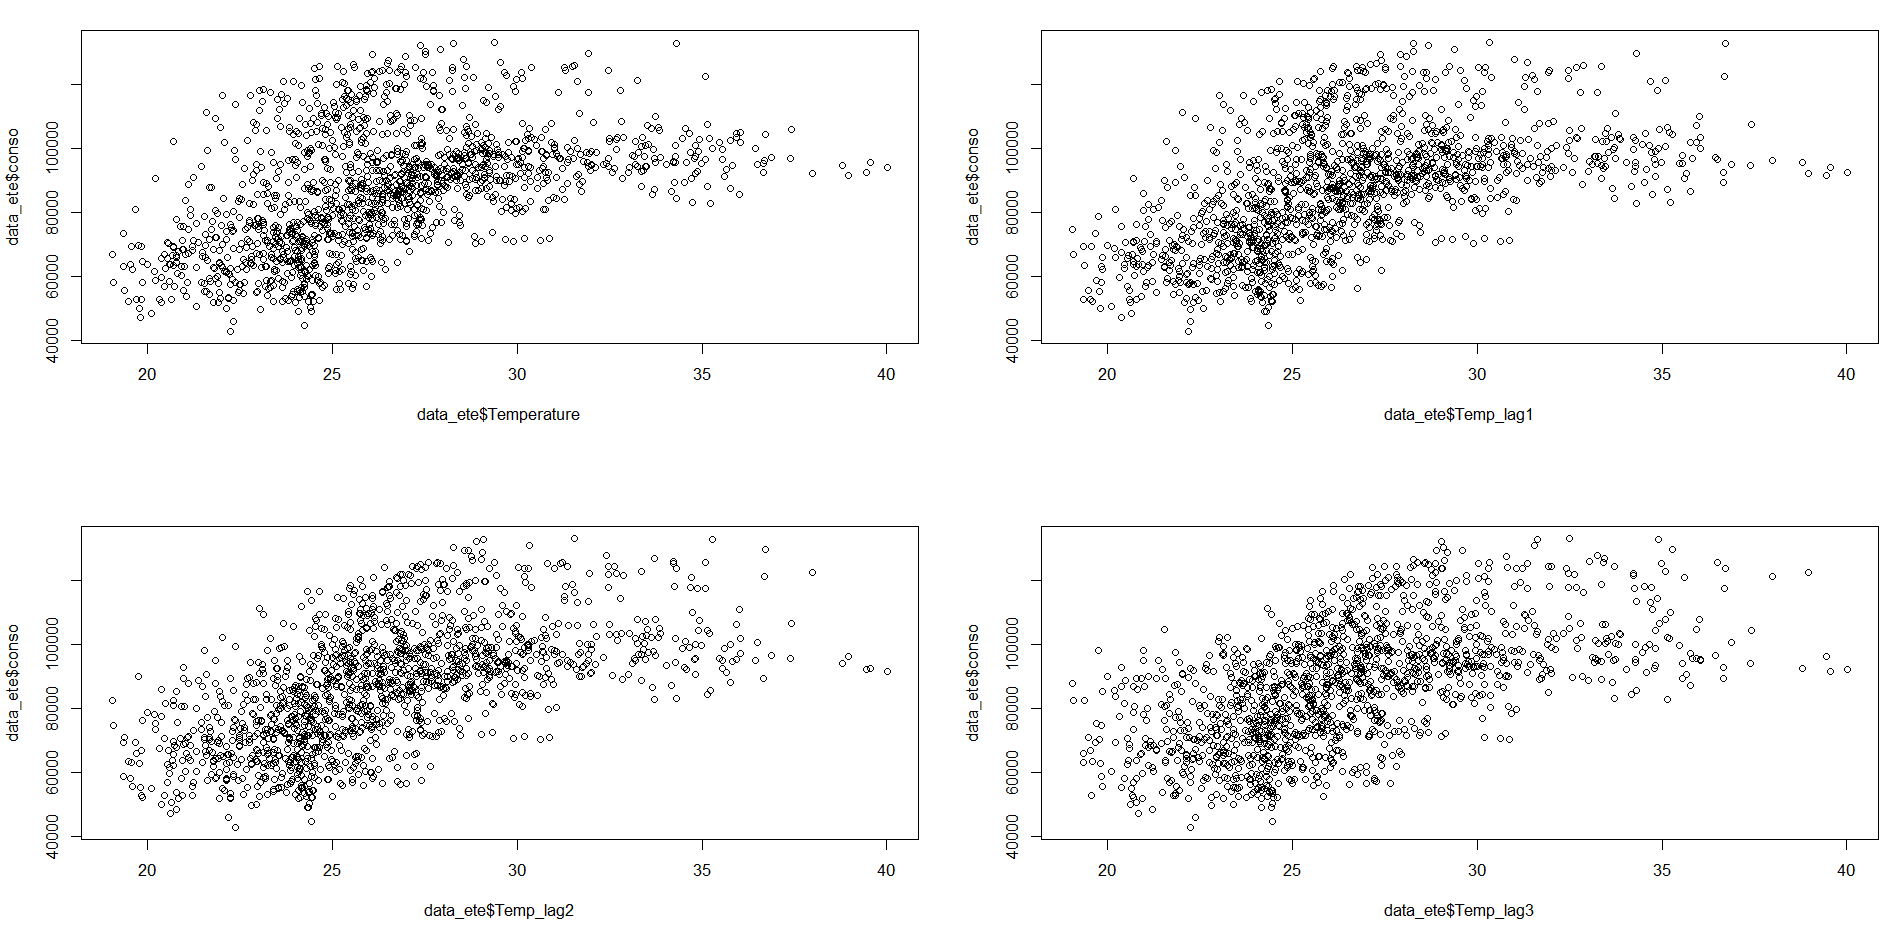
\includegraphics[width=0.75\linewidth]{fig12.png}
    \caption{Nuages de points associé à la consommation en fonction de la température pour différents décalages }
    \label{fig:enter-label}
\end{figure}

On observe que la corrélation entre la consommation et la température sans décalage ou avec un décalage d'une, deux ou trois heures sont respectivement de 0.481, 0.543, 0.574 et 0.575. La corrélation entre la consommation électrique est donc modérée surtout après un décalage de deux ou trois heures.\newline
On peut aussi évaluer la part de variance de la consommation électrique expliquée par la température grâce aux $R^2$ ajustés associés aux modèle linéaires de la consommation en fonction de la température sans décalage ou avec un décalage d'une, deux ou trois heures. On obtient des $R^2$ ajustés respectifs de 0.231, 0.294, 0.329 et 0.33. Ainsi, la température avec un décalage de trois heures expliquent le plus de variance ($33\%$). \newline
Lorsque l'on regarder le modèle $conso\sim Temperature+temp_{lag1}+temp_{lag2}+temp_{lag3}$, on obtient un $R^2$ ajusté de 0.34 ; la quasi-totalité de la variance expliquée par $Temperature$, $temp_{lag1}$ et $temp_{lag2}$ est donc contenue dans la variance expliquée par $temp_{lag3}$.\newline \\
Pour finir, on va étudier la corrélation entre les résidus du modèle SARIMA manuel associé à la consommation et la température à trois heures de décalage. Si cette corrélation s'avère significative, on va pouvoir améliorer le modèle SARIMA manuel en ajoutant une variable explicative (modèle SARIMAX). \newpage
Commençons par tracer le nuage de point associé aux résidus du modèle manuel en fonction de la température (toujours avec un décalage de trois heures).
\FloatBarrier
\begin{figure}[!h]
    \centering
    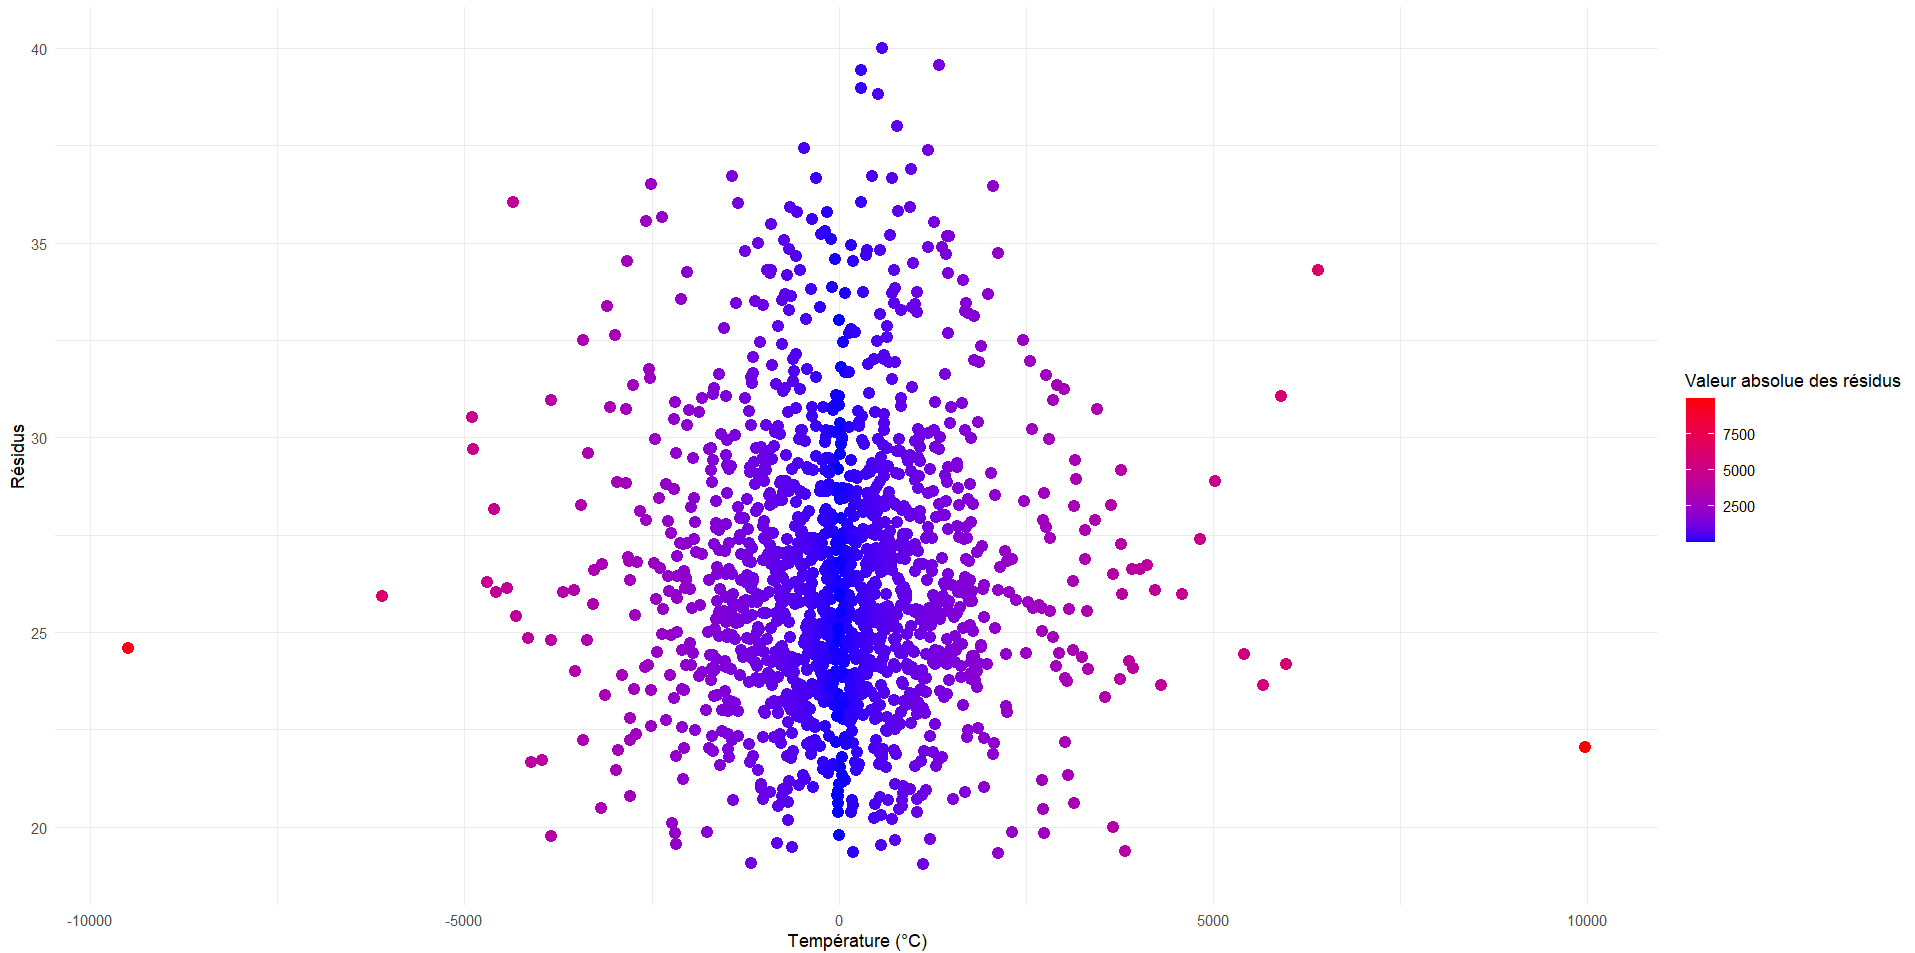
\includegraphics[width=0.8\linewidth]{figterm.png}
    \caption{\centering Nuage de points associé aux résidus du modèle SARIMA en fonction de la température à trois heures de décalage}
    \label{fig:enter-label}
\end{figure}
On remarque une concentration des points au voisinage du point (0,25). Cela est du au fait que la température moyenne l'été est proche de 25 et que le modèle SARIMA est bien ajusté (erreur moyenne relative de 0).\newline
De plus, la distribution des résidus à température fixée à l'air à peu près identique (le fait qu'il existe des points plus rouges lorsque la température est proche de 25°C vient du fait qu'il y a plus d'observations sous cette température).\newline
Ainsi, on peut conjecturer que la température n'influence pas les résidus du modèle ; i.e. l'information transmise par la température à trois heures de décalage est résumée dans le modèle manuel.\newline
Pour vérifier ce dernier point, on calcule la corrélation entre la température (à trois heures de décalage) et les résidus du modèle manuel. On obtient une corrélation trsè faible de $8.45.10^{-5}$. 
\newline
\\
Par conséquent, la température, notamment celle à trois heures de décalage, est corrélée de manière modérée avec la consommation électrique mais le modèle construit manuellement afin de prédire la consommation électrique en tient compte indirectement.

\section*{Conclusion}
Cette étude a permis de modéliser la consommation électrique et la température estivales à Tétouan à l'aide de modèles SARIMA et de lissage exponentiel, tout en explorant leur corrélation.

\subsection*{Modélisation de la température}
Le modèle SARIMA(2,0,0)(1,1,1)[24], conçu manuellement, s'est avéré optimal pour prédire les variations de température :
\begin{itemize}
    \item Critères d'information : Avec un AIC de 3158.98 et un BIC de 3185.42, il surpasse l'Auto-SARIMA (AIC = 3421.59) et l'ETS (AIC = 9857.85), indiquant un meilleur équilibre entre précision et parcimonie.
    \item Structure adaptée : Il capture efficacement la saisonnalité journalière (24h) et les fluctuations résiduelles, comme en témoignent les résidus stationnaires (test KPSS non significatif) et l'absence d'autocorrélation (test de Box-Ljung validé).
    \item Performance en prévision : Bien que le modèle ETS (RMSE moyen = 1.58) soit légèrement plus précis à court terme (J+1 à J+3), le SARIMA manuel offre une robustesse supérieure à moyen terme (J+4 à J+7) grâce à sa capacité à modéliser explicitement les dépendances temporelles complexes.
\end{itemize}
\subsection*{Modélisation de la consommation électrique}
Le SARIMA(1,1,0)(1,1,1)[24] manuel est retenu pour la prévision de la consommation :
\begin{itemize}
    \item Avantages statistiques : Ses critères AIC (25054) et BIC (25070) sont nettement inférieurs à ceux de l'ETS (AIC = 32443.88), validant sa supériorité en termes d'ajustement.
    \item Précision à court terme : Il minimise l'erreur (RMSE moyen = 7915 sur J+1 à J+4) comparé à l'ETS (RMSE moyen = 10030), grâce à la différenciation saisonnière et non saisonnière, essentielle pour gérer la tendance décroissante en août.
    \item Limitations à long terme : Au-delà de J+4, tous les modèles voient leur erreur augmenter, mais le SARIMA reste préférable pour son interprétabilité et sa structure paramétrique claire.
\end{itemize}
\subsection*{Corrélation température-consommation}
Bien qu'une corrélation modérée ($R^2 = 33\%$), existe entre la consommation et la température décalée de 3 heures, les résidus du SARIMA ne présentent aucune dépendance significative avec cette variable ($r = 8.45*10^-5$). Cela suggère que le modèle SARIMA intègre déjà indirectement l'effet de la température via ses composantes autorégressives et saisonnières, rendant superflu l'ajout d'une régresseur externe (SARIMAX).
\subsection*{Synthèse des choix}
\FloatBarrier
\begin{figure}[!h]
    \centering
    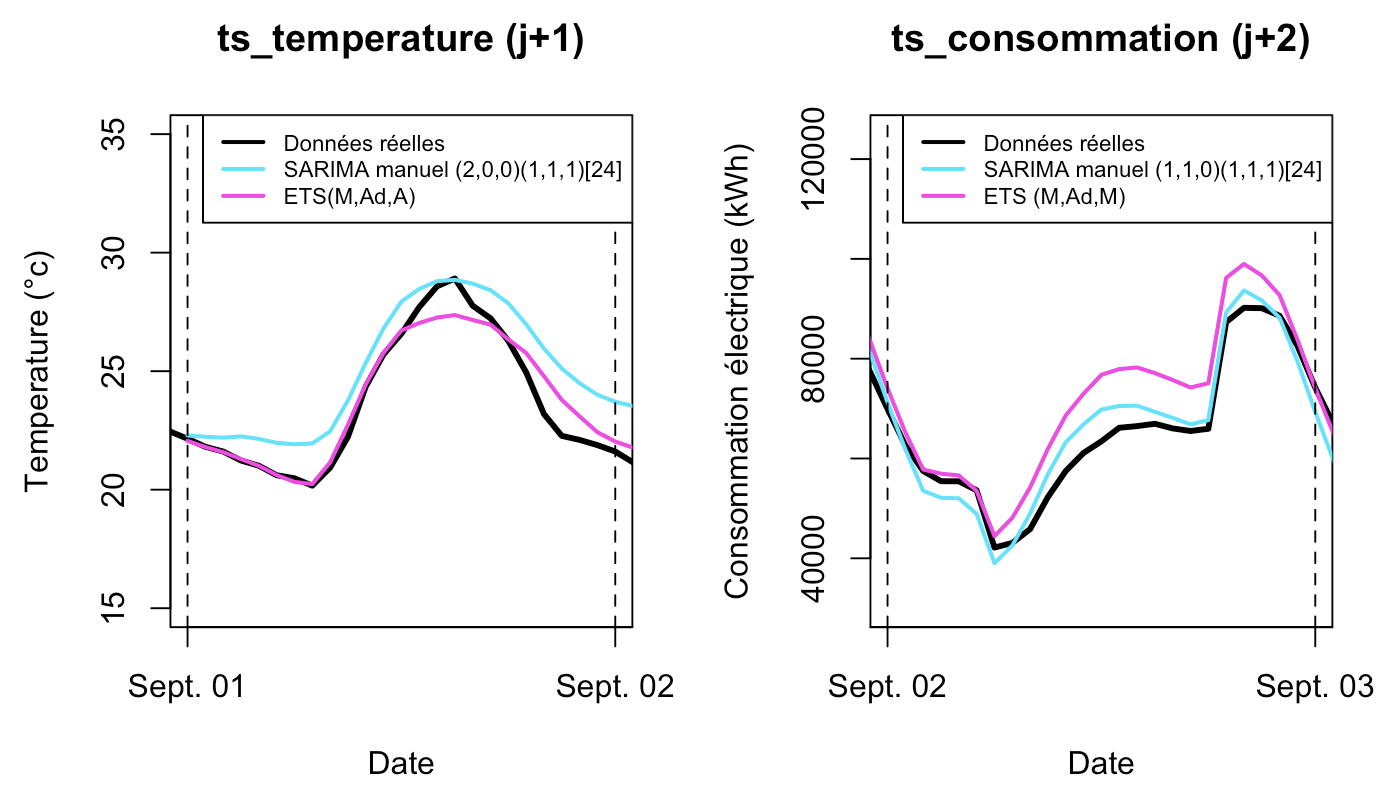
\includegraphics[width=0.8\linewidth]{concl.png}
    \caption{\centering Comparaison des modeles pour les séries ts\_temp et ts\_conso}
    \label{fig:enter-label}
\end{figure}

\begin{itemize}
    \item Température : Le SARIMA manuel est retenu pour sa capacité à capter le pic-saissonier à j+1, la prévision des pics etant plus important que celle des températures en heures creuses (où ETS est + puissant) dans le cadre de notre analyse.
    \item Consommation : Le SARIMA manuel est privilégié pour les prévisions à J+1 à J+4 (fournit de meilleures estiamtions en moyenne avec un AIC très simmilaire au modèle automatique), tandis qu'une approche hybride (recalage quotidien du modèle) serait nécessaire au-delà.
\end{itemize}


Cette analyse souligne l'importance d'arbitrer entre complexité et interprétabilité, et confirme que les modèles SARIMA, bien paramétrés, restent pertinents pour des séries présentant des saisonnalités et des tendances marquées.
\end{document}
